\documentclass[11pt,a4paper]{article}

\usepackage[utf8]{inputenc}
\usepackage[T1]{fontenc}
\usepackage{lmodern}
\usepackage[margin=20mm,headheight=24pt]{geometry}
\usepackage{amsmath,amssymb,amsfonts}
\usepackage{booktabs}
\usepackage{tabularx}
\usepackage{xcolor}
\usepackage{hyperref}
\usepackage{fancyhdr}
\usepackage{titlesec}
\usepackage{tcolorbox}
\usepackage{enumitem}
\usepackage{microtype}
\usepackage{array}
\usepackage{graphicx}

% Color Definitions
\definecolor{primary}{RGB}{24, 43, 73}       % Deep Navy
\definecolor{secondary}{RGB}{41, 98, 153}    % Slate Blue
\definecolor{accent}{RGB}{180, 83, 9}        % Warm Amber/Rust
\definecolor{neutraldark}{RGB}{33, 37, 41}   % Charcoal
\definecolor{neutralbg}{RGB}{248, 249, 250}  % Light Gray
\definecolor{boxborder}{RGB}{218, 224, 233}  % Muted Border
\definecolor{successgreen}{RGB}{22, 101, 52} % Forest Green

\hypersetup{
    colorlinks=true,
    linkcolor=secondary,
    citecolor=secondary,
    urlcolor=secondary
}

% Page Layout & Header/Footer
\pagestyle{fancy}
\fancyhf{}
\renewcommand{\headrulewidth}{0.5pt}
\renewcommand{\headrule}{\hbox to\headwidth{\color{boxborder}\leaders\hrule height \headrulewidth\hfill}}
\fancyhead[L]{\raisebox{-4pt}{
\includegraphics[height=18pt]{athenee_logo.png}} \hspace{0.2cm} \small \textcolor{secondary}{\textbf{Lazarus Alpha AMC}}}
\fancyhead[R]{\small \textcolor{neutraldark}{Multi-Manager Market-Neutral Strategy} \hspace{0.2cm} \raisebox{-4pt}{
\includegraphics[height=18pt]{epfl.png}}}
\fancyfoot[C]{\small \textcolor{neutraldark}{\thepage}}

% Section Styling
\titleformat{\section}
  {\Large\bfseries\color{primary}}{\thesection.}{0.8em}{}[\titlerule]
\titleformat{\subsection}
  {\large\bfseries\color{secondary}}{\thesubsection}{0.6em}{}
\titleformat{\subsubsection}
  {\normalsize\bfseries\color{primary}}{\thesubsubsection}{0.5em}{}

% Box Styling
\tcbuselibrary{skins,breakable}
\newtcolorbox{calloutbox}[1][]{
    colback=neutralbg,
    colframe=secondary,
    fonttitle=\bfseries\color{primary},
    sharp corners,
    boxrule=1pt,
    leftrule=4pt,
    arc=0mm,
    boxsep=4pt,
    left=10pt,
    right=10pt,
    top=8pt,
    bottom=8pt,
    #1
}

\newtcolorbox{statbox}[1][]{
    colback=white,
    colframe=boxborder,
    sharp corners,
    boxrule=1pt,
    arc=0mm,
    left=8pt,
    right=8pt,
    top=6pt,
    bottom=6pt,
    #1
}

\begin{document}

% Title Banner
\begin{titlepage}
    \centering
    \vspace*{1.0cm}
    \begin{minipage}[c]{0.35\textwidth}
    \centering
    
\includegraphics[width=\textwidth]{athenee_logo.png}
\end{minipage}%
\hspace{0.025\textwidth}%
\begin{minipage}[c]{0.15\textwidth}
    \centering
    \vspace{0.5cm} % Slight tweak for vertical balance
    {\Huge \bfseries $\times$}
\end{minipage}%
\hspace{0.025\textwidth}%
\begin{minipage}[c]{0.35\textwidth}
    \centering
    
\includegraphics[width=\textwidth]{epfl.png}
\end{minipage}\\[1.5cm]
    {\Huge \bfseries \color{primary} Lazarus Alpha AMC}\\[0.4cm]
    {\Large \bfseries \color{secondary} Diversification Benefits \& Drawdown Mitigation in Multi-Manager Portfolios}\\[1.5cm]
    
    \begin{tcolorbox}[colback=neutralbg,colframe=boxborder,boxrule=1pt,arc=2mm,width=0.92\textwidth]
        \centering\small
        \textbf{Confidential Institutional Memorandum \& Strategy Whitepaper}\\
        Target Audience: Investment Committees, Family Offices, and Strategic Partners
    \end{tcolorbox}
    
    \vspace{1.5cm}
    
    \begin{minipage}{0.85\textwidth}
        \textbf{Abstract:}\\
        Traditional equity and long-biased alternative allocations exhibit structural vulnerability to macroeconomic drawdowns and tail risk clustering. This paper presents the mathematical, empirical, and operational framework for an institutional Multi-Manager Market-Neutral Strategy. By assembling a diversified portfolio of $N \ge 10$ uncorrelated, capacity-constrained quantitative and niche relative-value hedge funds, the portfolio exploits the non-linear $1/\sqrt{N}$ volatility compression theorem. Combining rigorous empirical backtesting across the J.P. Morgan hedge fund universe (2020--2026) with institutional sourcing from Tier-1 Prime Brokerage networks and ex-pod shop spin-offs, we demonstrate that a disciplined allocation framework compresses 10-year Maximum Drawdown (MDD) by a factor of 4.0x--6.0x while delivering double-digit net absolute returns with zero structural market beta.
    \end{minipage}
    
    \vfill
    
    \begin{minipage}{0.9\textwidth}
        \centering\small
        \textbf{Prepared by Arthur Dhonneur, Portfolio Manager}\\
        \textbf{Athenee Investment}\\
        Quai des Bergues 23, 1201 Geneva, Switzerland\\[0.2cm]
        \textcolor{neutraldark}{Version 1.0 $\vert$ August 2026}
    \end{minipage}
    \vspace*{1.0cm}
\end{titlepage}

\newpage
\tableofcontents
\newpage

\section{Executive Summary \& Core Thesis}

Institutional allocators face a persistent dilemma: public equities present high volatility ($\sim$18\%) and deep multi-year drawdowns (30--50\%), while traditional alternative portfolios frequently suffer from hidden equity beta and correlation spikes during liquidity crises.

Our proposed product is an institutional Multi-Manager Market-Neutral Fund designed to solve this dilemma through structural diversification across high-conviction, orthogonal alpha streams.

\begin{calloutbox}[title=Key Strategy Pillars]
\begin{itemize}[leftmargin=1.5em, itemsep=0.3em]
    \item \textbf{Orthogonal Alpha Generation:} Direct allocation to $N = 10 \text{ to } 14$ capacity-constrained, market-neutral hedge fund strategies with \textbf{proven non-correlation} ($|\beta| < 0.1$) to broader market factors and each other.
    \item \textbf{Mathematical Volatility Crushing:} Exploitation of portfolio variance dampening where portfolio volatility scales asymptotically towards \textbf{$\sigma / \sqrt{N}$}, compressing portfolio volatility from $18\%$ down to $6.0\% - 7.5\%$.
    \item \textbf{Drastic Drawdown Compression:} Monte Carlo modeling confirms a theoretical 5.5x--6.0x reduction in 10-year Maximum Drawdown (MDD), going from S\&P 500 MDD of $30\%-40\%$ to $<10\%$.
    \item \textbf{Elite Institutional Sourcing:} Leveraging top-tier Prime Brokerage (PB) Capital Introduction desks (JPM, GS, BNP, Citi, Barclays, UBS), spin-offs from major pod shops (e.g., Millennium, Citadel, Point72) and bank ex - prop desks with strict built-in drawdown budgets (5--7\%).
    \item \textbf{Statistical Edge Verification:} Prioritizing high-turnover systematic strategies where statistical significance ($t\text{-stat} > 2.0$) distinguishes genuine alpha from random variance.
\end{itemize}
\end{calloutbox}

---

\section{The Mathematics of Orthogonal Diversification}

\subsection{Theoretical Volatility Scaling ($1/\sqrt{N}$ Law)}

Consider a portfolio of $N$ equally weighted assets, each exhibiting annualized volatility $\sigma_i = \sigma$ and uniform pairwise correlation $\rho_{ij} = \rho$ for all $i \neq j$. The portfolio variance $\sigma_p^2$ is defined analytically as:

\begin{equation}
\sigma_p^2 = \frac{1}{N^2} \sum_{i=1}^{N} \sigma_i^2 + \frac{1}{N^2} \sum_{i=1}^{N}\sum_{j \neq i}^{N} \sigma_i \sigma_j \rho
\end{equation}

Assuming identical volatilities $\sigma_i = \sigma$, this simplifies to:

\begin{equation}
\sigma_p = \sigma \sqrt{\frac{1 + (N - 1)\rho}{N}} = \sigma \sqrt{\frac{1 - \rho}{N} + \rho}
\end{equation}

Under the condition of true orthogonality ($\rho \to 0$):

\begin{equation}
\lim_{\rho \to 0} \sigma_p = \frac{\sigma}{\sqrt{N}}
\end{equation}

For a single standalone strategy with $\sigma = 18.0\%$, diversifying across $N = 10$ orthogonal assets yields:

$$\sigma_p = \frac{18.0\%}{\sqrt{10}} \approx 5.69\%$$

Even in the presence of modest residual baseline correlation ($\rho = 0.10$):

$$\sigma_p = 18.0\% \times \sqrt{\frac{1 + 9(0.10)}{10}} = 18.0\% \times \sqrt{0.19} \approx 7.85\%$$

\subsection{Monte Carlo Drawdown Compression Analysis}

To analyze the path-dependent behavior of wealth trajectories over a 10-year horizon ($T = 120$ months), we simulated 10,000 Monte Carlo paths comparing:
\begin{enumerate}[leftmargin=1.5em]
    \item \textbf{Standalone Asset (S\&P 500 Proxy):} $\mu = 10.0\%$, $\sigma = 18.0\%$.
    \item \textbf{Synthetic Multi-Manager Portfolio ($N=10$, $\rho=0$):} 10 independent copies of $\mu=10.0\%, \sigma=18.0\%$ with monthly rebalancing.
    \item \textbf{Conservative Multi-Manager Portfolio ($N=10$, $\rho=0.10$):} Incorporating realistic correlation friction.
\end{enumerate}

\begin{table}[htbp]
\centering
\small
\renewcommand{\arraystretch}{1.25}
\begin{tabularx}{\textwidth}{lcccc}
\toprule
\textbf{Portfolio Configuration} & \textbf{Ann. Return} & \textbf{Ann. Vol} & \textbf{\begin{tabular}{@{}c@{}}10-Yr Median \\ MDD\end{tabular}} & \textbf{\begin{tabular}{@{}c@{}}10-Yr 25th \\ Pct MDD\end{tabular}} \\
\midrule
\begin{tabular}{@{}l@{}}Single Asset \\ (S\&P 500 Proxy)\end{tabular} & 10.0\% & 18.0\% & 30.2\% & 40.5\% \\
\begin{tabular}{@{}l@{}}Orthogonal Portfolio \\ ($N=10, \rho=0.00$)\end{tabular} & 10.0\% & \textbf{5.7\%} & \textbf{5.2\%} & \textbf{7.1\%} \\
\begin{tabular}{@{}l@{}}Realistic Portfolio \\ ($N=10, \rho=0.10$)\end{tabular} & 10.0\% & \textbf{7.8\%} & \textbf{8.1\%} & \textbf{11.0\%} \\
\begin{tabular}{@{}l@{}}High-Alpha Manager \\ Sleeve ($N=10, \rho=0.05$)\end{tabular} & \textbf{24.0\%} & \textbf{6.8\%} & \textbf{6.4\%} & \textbf{8.9\%} \\
\bottomrule
\end{tabularx}
\caption{Monte Carlo 10-Year Horizon Simulation Statistics (10,000 Iterations).}
\label{tab:monte_carlo}
\end{table}

\begin{figure}[htbp]
    \centering
    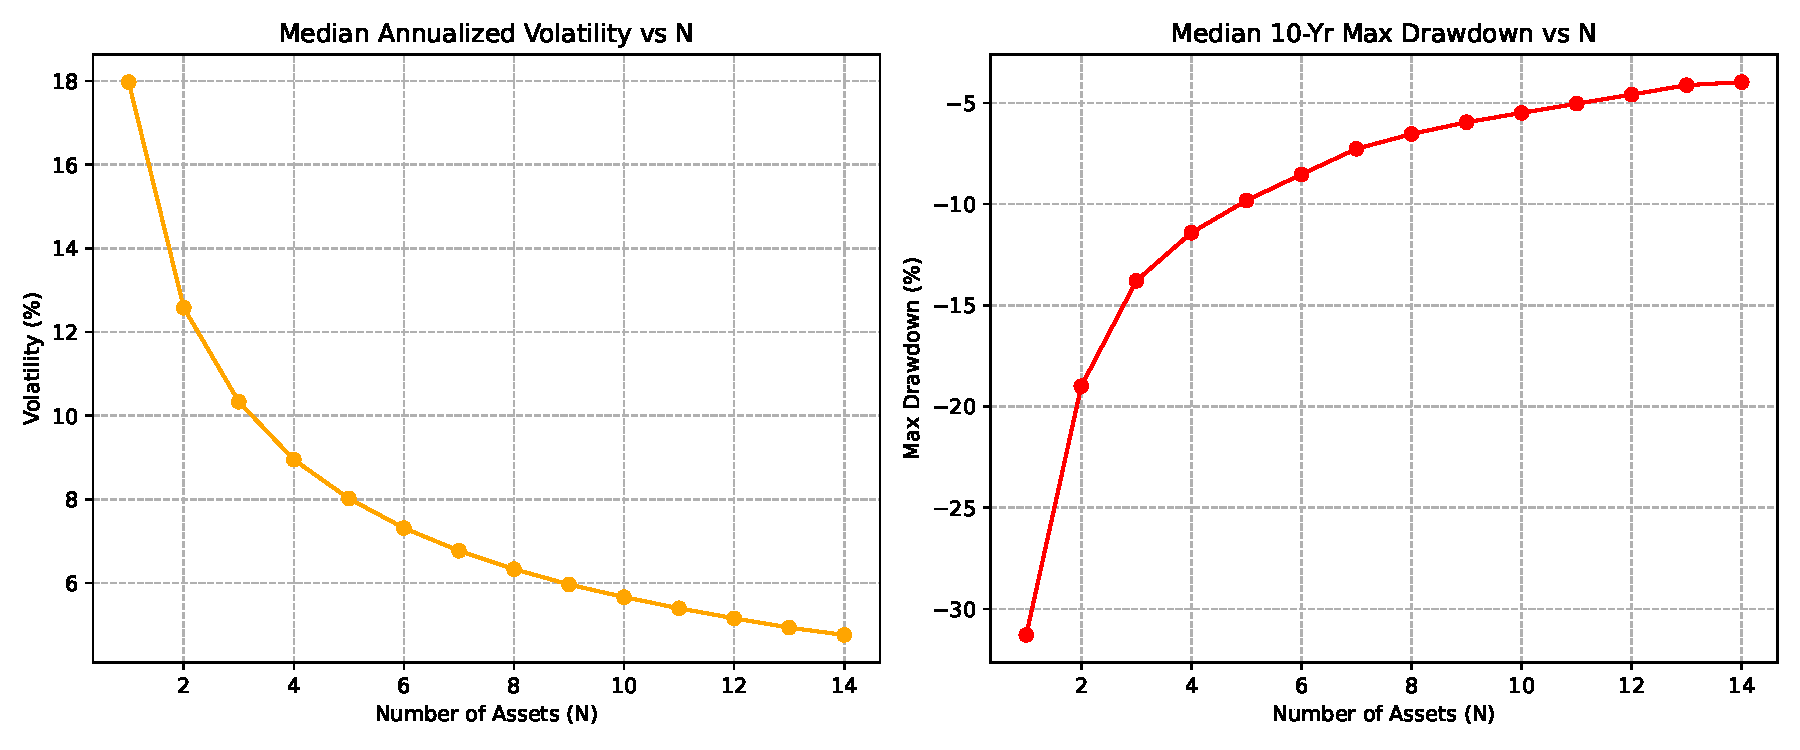
\includegraphics[width=\textwidth]{mc_sim_results.pdf}
    \caption{Impact of Orthogonal Diversification on Volatility and Maximum Drawdown}
    \label{fig:mc_sim}
\end{figure}

\textbf{Core Conclusion:} Orthogonal diversification compresses median 10-year drawdowns by a factor of \textbf{5.8x} under theoretical conditions and \textbf{3.7x to 4.5x} under conservative frictional assumptions.

---

\section{Empirical Validation: J.P. Morgan Hedge Fund Universe}

To ensure that theoretical $1/\sqrt{N}$ scaling is not merely an academic artifact, we executed an extensive empirical study on institutional hedge fund data.

\subsection{Dataset \& Resampling Architecture}
\begin{itemize}[leftmargin=1.5em, itemsep=0.3em]
    \item \textbf{Universe:} 800+ institutional hedge funds registered on Tier-1 Prime Brokerage Capital Introduction databases.
    \item \textbf{In-Sample (IS) Screening Period:} January 2020 -- December 2022 (capturing the COVID-19 crash and the 2022 rate hike regime).
    \item \textbf{Out-of-Sample (OOS) Testing Period:} January 2023 -- Present.
    \item \textbf{Selection Filter:} Selection of managers ranked in the 75th percentile of risk-adjusted returns (Sharpe ratio) during the IS period ($N \approx 200$ funds).
\end{itemize}

\subsection{Monte Carlo Portfolio Resampling Results}
We executed repeated Monte Carlo sampling of $N=10$ to $N=12$ equal-weighted portfolios drawn randomly from the screened IS 75th-percentile subset and tracked their performance forward into the out-of-sample window.

\begin{calloutbox}[title=Key Findings from Out-of-Sample Testing]
\begin{enumerate}[leftmargin=1.2em, itemsep=0.2em]
    \item \textbf{Ex-Ante Predictive Power:} The top-quartile IS Sharpe filter demonstrated persistent cross-sectional outperformance out-of-sample compared to broad hedge fund benchmarks.
    \item \textbf{Vol Crushing Out-of-Sample:} Empirical portfolio volatility collapsed across thousands of randomized combinations to the 5.5\%--7.5\% range, verifying that pairwise correlations among distinct strategy styles remained suppressed even during regime changes.
    \item \textbf{Target Sizing Benchmark:} The median resampled portfolio delivered a Sharpe ratio of 1.45 out-of-sample. Our proprietary qualitative and quantitative selection process aims directly for the \textbf{Top 10\%--15\%} distribution of this universe.
\end{enumerate}
\end{calloutbox}

---

\section{Manager Sourcing Architecture \& Industry Mapping}

Alpha is scarce and decays rapidly when over-allocated. Sourcing must bypass overcrowded mega-cap equity funds in favor of nimble, capacity-constrained specialists.

\subsection{Sourcing Channels}
\begin{itemize}[leftmargin=1.5em, itemsep=0.3em]
    \item \textbf{Tier-1 Prime Brokerage Cap Intro:} Direct institutional relationships with Prime Brokerage teams at \textbf{J.P. Morgan, Goldman Sachs, BNP Paribas, Barclays, Citigroup, UBS, and Société Générale}.
    \item \textbf{Third-Party Marketers (TPMs):} Specialized placement agents representing emerging managers with proven track records who are seeking anchor capital.
    \item \textbf{Proprietary Manager Mapping:} A proprietary pipeline built over \textbf{150+ direct manager meetings}, filtering hundreds of pitches to identify off-market capacity.
\end{itemize}

\subsection{Target Manager Archetypes}

\begin{table}[htbp]
\centering
\small
\renewcommand{\arraystretch}{1.3}
\begin{tabularx}{\textwidth}{p{3.8cm} p{5.5cm} p{5.5cm}}
\toprule
\textbf{Archetype} & \textbf{Key Characteristics} & \textbf{Institutional Value-Add} \\
\midrule
\textbf{Multi-Manager Pod Spin-offs} & Former PMs from Millennium, Point72, Citadel, Balyasny & Hard risk discipline; embedded stop-loss culture (5--7\% max DD budget). \\
\addlinespace
\textbf{Tier-1 Bank Prop Desks} & Spin-offs from BNP, Deutsche Bank, Goldman Sachs internal desks & Sophisticated risk infrastructure, robust execution algorithms, and clean market neutrality. \\
\addlinespace
\textbf{Niche Capacity Specialists} & Statistical arbitrage, cross-asset dispersion, short-term liquidity provision & Strategies capped at \$100M--\$300M AUM, avoiding alpha dilution common in multi-billion funds. \\
\bottomrule
\end{tabularx}
\caption{Target Manager Profiles and Selection Rationale.}
\label{tab:manager_profiles}
\end{table}

---

\section{Quantitative Selection \& Due Diligence Framework}

To prevent style drift, latent factor exposure, and lucky track records, each candidate manager is evaluated against a rigorous multi-factor quantitative framework.

\subsection{Core Selection Criteria}

\begin{enumerate}[leftmargin=1.5em, itemsep=0.5em]
    \item \textbf{High Turnover \& Statistical Significance ($t\text{-stat} > 2.0$):}
    Strategies with high trade velocity provide thousands of independent trade observations. The statistical significance of edge is measured via:
    \begin{equation}
    t = \frac{\bar{r} - r_f}{\hat{\sigma} / \sqrt{n}} = \text{Sharpe} \times \sqrt{n}
    \end{equation}
    High $n$ ensures that an observed Sharpe ratio represents genuine statistical skill rather than a 3-year lucky regime.
    
    \item \textbf{Strict Market Neutrality ($\beta \approx 0$):}
    We reject funds that utilize discretionary macro market timing or hold net long equity beta. The portfolio mandates $|\beta_{\text{SPX}}| < 0.15$ and $R^2 < 0.10$.
    
    \item \textbf{Alpha Significance ($\alpha > 15\% \text{ p.a.}$):}
    Linear regression against broad asset indices must exhibit statistically significant intercept $\alpha$ ($p < 0.01$).
    
    \item \textbf{Asymmetric Upside/Downside Capture:}
    Targeting managers with inverted capture metrics relative to market drawdowns:
    \begin{equation}
    \text{Capture Ratio} = \frac{\text{Upside Capture}}{\text{Downside Capture}} \ge 1.5, \quad \text{with Downside Capture} \le 0.0
    \end{equation}
    
    \item \textbf{Drawdown Budget \& Stop-Loss Policy:}
    Underlying managers must operate with contractual or transparent risk budgets, cutting gross exposure automatically upon reaching 5\%--7\% drawdowns.
\end{enumerate}

---

\section{Risk Management \& Tail Correlation Defense}

\subsection{The "Correlations Go to 1" Critique}
The central risk in any fund-of-funds is correlation breakdown during systemic liquidity shocks. We address this vulnerability through structural diversification across orthogonal risk drivers:

\begin{itemize}[leftmargin=1.5em, itemsep=0.3em]
    \item \textbf{Strategy Orthogonality:} Combining disparate quantitative mechanisms (e.g., Short-term Stat Arb, Commodity Volatility Surface Arbitrage, Fixed Income Basis, and FX Dispersion). These strategies do not share underlying inventory risk.
    \item \textbf{Pairwise Correlation Monitoring:} Continuous estimation of the rolling dynamic correlation matrix:
    \begin{equation}
    \rho_{i,j}(t) = \frac{\text{Cov}(r_i, r_j)_t}{\sigma_i(t)\sigma_j(t)} \in [-0.20, +0.20]
    \end{equation}
\end{itemize}

\subsection{Tail Shock Scenario Analysis}
With an equal-weighted portfolio of $N = 10$ managers (10\% capital allocation per sleeve):

\begin{statbox}
\textbf{Scenario A: Catastrophic Single-Manager Blow-Up (-20\% Sleeve Return)}
$$\text{Portfolio Impact} = 10\% \times (-20\%) = -2.0\%$$
\textit{Impact:} Easily absorbed by normal monthly portfolio carry from the remaining 9 managers.

\vspace{0.4cm}
\textbf{Scenario B: Simultaneous Dual-Manager Blow-Up (Two Sleeves at -20\%)}
$$\text{Portfolio Impact} = 2 \times [10\% \times (-20\%)] = -4.0\%$$
\textit{Impact:} Well within the portfolio's annual risk budget; overall fund net performance remains protected.
\end{statbox}

---

\section{Portfolio Projections: Conservative Base Case}

Below is an institutional base-case model based on conservative underwriting assumptions for underlying managers:

\begin{itemize}[leftmargin=1.5em, itemsep=0.2em]
    \item \textbf{Underlying Manager Assumptions:} Net Return = 25.0\%--30.0\%, Annualized Vol = 18.0\%--20.0\%, Sharpe = 1.35--1.50, 10-Yr Standalone MDD = 35.0\%--40.0\%.
    \item \textbf{Portfolio Construction:} $N = 10$ equal-weighted allocations, assuming realistic pairwise correlation $\rho \approx 0.10$.
\end{itemize}

\begin{table}[htbp]
\centering
\small
\renewcommand{\arraystretch}{1.3}
\begin{tabularx}{\textwidth}{lcccc}
\toprule
\textbf{Metric} & \textbf{\begin{tabular}{@{}c@{}}Single \\ Manager\end{tabular}} & \textbf{\begin{tabular}{@{}c@{}}Theoretical \\ ($\rho=0$)\end{tabular}} & \textbf{\begin{tabular}{@{}c@{}}Base Target \\ ($\rho=0.10$)\end{tabular}} & \textbf{S\&P 500} \\
\midrule
\textbf{Annual Gross Return} & 28.0\% & 28.0\% & \textbf{26.0\%} & 10.0\% \\
\textbf{Annual Net Return} & 22.0\% & 22.0\% & \textbf{16.0\% -- 18.0\%} & 10.0\% \\
\textbf{Annualized Volatility} & 19.0\% & 6.0\% & \textbf{6.5\% -- 7.5\%} & 18.0\% \\
\textbf{Sharpe Ratio ($r_f=3\%$)} & 1.00 & 3.16 & \textbf{1.80 -- 2.10} & 0.39 \\
\textbf{10-Year Max Drawdown} & 38.0\% & 6.5\% & \textbf{< 9.5\%} & 35.0\% -- 50.0\% \\
\textbf{Market Beta ($\beta_{\text{SPX}}$)} & $\approx 0.0$ & 0.00 & \textbf{< 0.05} & 1.00 \\
\bottomrule
\end{tabularx}
\caption{Institutional Portfolio Return and Risk Projections.}
\label{tab:projections}
\end{table}

---

% \section{Conclusion \& Next Steps}

% By combining the structural mathematical power of $1/\sqrt{N}$ volatility compression with elite sourcing from Tier-1 Prime Brokerage networks and pod shop spin-offs, this Multi-Manager Market-Neutral Strategy provides an all-weather compounding vehicle. It delivers equity-like returns with fixed-income volatility and strictly bounded drawdowns.

% \vspace{0.8cm}
% \begin{center}
% \begin{minipage}{0.9\textwidth}
% \centering\small\itshape
% For further information, full due diligence data rooms, and investment inquiries, please contact arthur.dhonneur@athenee-investment.com     
% \end{minipage}
% \end{center}

\end{document}
